%% Beginning of file 'sample631.tex'
%%
%% Modified 2021 March
%%
%% This is a sample manuscript marked up using the
%% AASTeX v6.31 LaTeX 2e macros.
%%
%% AASTeX is now based on Alexey Vikhlinin's emulateapj.cls 
%% (Copyright 2000-2015).  See the classfile for details.

%% AASTeX requires revtex4-1.cls and other external packages such as
%% latexsym, graphicx, amssymb, longtable, and epsf.  Note that as of 
%% Oct 2020, APS now uses revtex4.2e for its journals but remember that 
%% AASTeX v6+ still uses v4.1. All of these external packages should 
%% already be present in the modern TeX distributions but not always.
%% For example, revtex4.1 seems to be missing in the linux version of
%% TexLive 2020. One should be able to get all packages from www.ctan.org.
%% In particular, revtex v4.1 can be found at 
%% https://www.ctan.org/pkg/revtex4-1.

%% The first piece of markup in an AASTeX v6.x document is the \documentclass
%% command. LaTeX will ignore any data that comes before this command. The 
%% documentclass can take an optional argument to modify the output style.
%% The command below calls the preprint style which will produce a tightly 
%% typeset, one-column, single-spaced document.  It is the default and thus
%% does not need to be explicitly stated.
%%
%% using aastex version 6.3
\documentclass[linenumbers,twocolumn]{aastex631}
%\documentclass[linenumbers]{aastex631}
%\documentclass[linenumbers,twocolumn]%{aastex631}
\usepackage[dvipsnames]{xcolor}
\usepackage{color}
\usepackage{makecell}
\usepackage{appendix}
\usepackage{mathrsfs}
\usepackage{longtable}
\usepackage{hyperref}
\hypersetup{colorlinks=true, urlcolor=blue}
%\usepackage[UTF8,heading = true]{ctex}
\frenchspacing
\newcommand{\ud}{\mathrm{d}}
\newcommand{\dirac}{\partial\llap{$\diagup$\kern-2pt}}
\newcommand{\fett}[1]{\boldsymbol{#1}}
\newcommand{\fettu}[1]{\mathbf{#1}}
\newcommand{\quabla}{\square}
\newcommand{\diag}{\mathrm{diag}}
\newcommand{\sgn}{\mathrm{sgn}}
\newcommand{\Tr}{\mathrm{Tr}}
\newcommand{\Heaviside}{\theta}
\newcommand{\eig}{\mathrm{eig}}
\newcommand{\e}{\mathrm{e}}
%% The default is a single spaced, 10 point font, single spaced article.
%% There are 5 other style options available via an optional argument. They
%% can be invoked like this:
%%
%% \documentclass[arguments]{aastex631}
%% 
%% where the layout options are:
%%
%%  twocolumn   : two text columns, 10 point font, single spaced article.
%%                This is the most compact and represent the final published
%%                derived PDF copy of the accepted manuscript from the publisher
%%  manuscript  : one text column, 12 point font, double spaced article.
%%  preprint    : one text column, 12 point font, single spaced article.  
%%  preprint2   : two text columns, 12 point font, single spaced article.
%%  modern      : a stylish, single text column, 12 point font, article with
%% 		  wider left and right margins. This uses the Daniel
%% 		  Foreman-Mackey and David Hogg design.
%%  RNAAS       : Supresses an abstract. Originally for RNAAS manuscripts 
%%                but now that abstracts are required this is obsolete for
%%                AAS Journals. Authors might need it for other reasons. DO NOT
%%                use \begin{abstract} and \end{abstract} with this style.
%%
%% Note that you can submit to the AAS Journals in any of these 6 styles.
%%
%% There are other optional arguments one can invoke to allow other stylistic
%% actions. The available options are:
%%
%%   astrosymb    : Loads Astrosymb font and define \astrocommands. 
%%   tighten      : Makes baselineskip slightly smaller, only works with 
%%                  the twocolumn substyle.
%%   times        : uses times font instead of the default
%%   linenumbers  : turn on lineno package.
%%   trackchanges : required to see the revision mark up and print its output
%%   longauthor   : Do not use the more compressed footnote style (default) for 
%%                  the author/collaboration/affiliations. Instead print all
%%                  affiliation information after each name. Creates a much 
%%                  longer author list but may be desirable for short 
%%                  author papers.
%% twocolappendix : make 2 column appendix.
%%   anonymous    : Do not show the authors, affiliations and acknowledgments 
%%                  for dual anonymous review.
%%
%% these can be used in any combination, e.g.
%%
%% \documentclass[twocolumn,linenumbers,trackchanges]{aastex631}
%%
%% AASTeX v6.* now includes \hyperref support. While we have built in specific
%% defaults into the classfile you can manually override them with the
%% \hypersetup command. For example,
%%
%% \hypersetup{linkcolor=red,citecolor=green,filecolor=cyan,urlcolor=magenta}
%%
%% will change the color of the internal links to red, the links to the
%% bibliography to green, the file links to cyan, and the external links to
%% magenta. Additional information on \hyperref options can be found here:
%% https://www.tug.org/applications/hyperref/manual.html#x1-40003
%%
%% Note that in v6.3 "bookmarks" has been changed to "true" in hyperref
%% to improve the accessibility of the compiled pdf file.
%%
%% If you want to create your own macros, you can do so
%% using \newcommand. Your macros should appear before
%% the \begin{document} command.
%%
\newcommand{\vdag}{(v)^\dagger}
\newcommand\aastex{AAS\TeX}
\newcommand\latex{La\TeX}
\usepackage{amsmath}

%% Reintroduced the \received and \accepted commands from AASTeX v5.2
%\received{March 1, 2021}
%\revised{April 1, 2021}
%\accepted{\today}

%% Command to document which AAS Journal the manuscript was submitted to.
%% Adds "Submitted to " the argument.
%\submitjournal{PSJ}

%% For manuscript that include authors in collaborations, AASTeX v6.31
%% builds on the \collaboration command to allow greater freedom to 
%% keep the traditional author+affiliation information but only show
%% subsets. The \collaboration command now must appear AFTER the group
%% of authors in the collaboration and it takes TWO arguments. The last
%% is still the collaboration identifier. The text given in this
%% argument is what will be shown in the manuscript. The first argument
%% is the number of author above the \collaboration command to show with
%% the collaboration text. If there are authors that are not part of any
%% collaboration the \nocollaboration command is used. This command takes
%% one argument which is also the number of authors above to show. A
%% dashed line is shown to indicate no collaboration. This example manuscript
%% shows how these commands work to display specific set of authors 
%% on the front page.
%%
%% For manuscript without any need to use \collaboration the 
%% \AuthorCollaborationLimit command from v6.2 can still be used to 
%% show a subset of authors.
%
%\AuthorCollaborationLimit=2
%
%% will only show Schwarz & Muench on the front page of the manuscript
%% (assuming the \collaboration and \nocollaboration commands are
%% commented out).
%%
%% Note that all of the author will be shown in the published article.
%% This feature is meant to be used prior to acceptance to make the
%% front end of a long author article more manageable. Please do not use
%% this functionality for manuscripts with less than 20 authors. Conversely,
%% please do use this when the number of authors exceeds 40.
%%
%% Use \allauthors at the manuscript end to show the full author list.
%% This command should only be used with \AuthorCollaborationLimit is used.

%% The following command can be used to set the latex table counters.  It
%% is needed in this document because it uses a mix of latex tabular and
%% AASTeX deluxetables.  In general it should not be needed.
%\setcounter{table}{1}

%%%%%%%%%%%%%%%%%%%%%%%%%%%%%%%%%%%%%%%%%%%%%%%%%%%%%%%%%%%%%%%%%%%%%%%%%%%%%%%%
%%
%% The following section outlines numerous optional output that
%% can be displayed in the front matter or as running meta-data.
%%
%% If you wish, you may supply running head information, although
%% this information may be modified by the editorial offices.
\shorttitle{ Gaps in Prompt high-energy emission }
%\shortauthors{X.-Y. Song et al. }


%%
%% You can add a light gray and diagonal water-mark to the first page 
%% with this command:
%% \watermark{text}
%% where "text", e.g. DRAFT, is the text to appear.  If the text is 
%% long you can control the water-mark size with:
%% \setwatermarkfontsize{dimension}
%% where dimension is any recognized LaTeX dimension, e.g. pt, in, etc.
%%
%%%%%%%%%%%%%%%%%%%%%%%%%%%%%%%%%%%%%%%%%%%%%%%%%%%%%%%%%%%%%%%%%%%%%%%%%%%%%%%%
\graphicspath{{./}{figures/}}
%% This is the end of the preamble.  Indicate the beginning of the
%% manuscript itself with \begin{document}.

\begin{document}
\title{
%The extraordinary prompt high-energy emission in GRB 210704A: nuclide absorption or multi-mechanism
%Anomalous prompt high-energy emission in GRB 210704A: resonant nuclide absorption versus multi-component emission mechanisms %by Ma
%Peculiar prompt high-energy emission in GRB 210704A: a possible resonant nuclide absorption process %by Song
Spectroscopic Signature of r-Process Nucleosynthesis in a Gamma-Ray Burst: \\ Possible Resonant Deuterium Absorption in GRB 210704A
}

%% LaTeX will automatically break titles if they run longer than
%% one line. However, you may use \\ to force a line break if
%% you desire. In v6.31 you can include a footnote in the title.

%% A significant change from earlier AASTEX versions is in the structure for 
%% calling author and affiliations. The change was necessary to implement 
%% auto-indexing of affiliations which prior was a manual process that could 
%% easily be tedious in large author manuscripts.
%%
%% The \author command is the same as before except it now takes an optional
%% argument which is the 16 digit ORCID. The syntax is:
%% \author[xxxx-xxxx-xxxx-xxxx]{Author Name}
%%
%% This will hyperlink the author name to the author's ORCID page. Note that
%% during compilation, LaTeX will do some limited checking of the format of
%% the ID to make sure it is valid. If the "orcid-ID.png" image file is 
%% present or in the LaTeX pathway, the OrcID icon will appear next to
%% the authors name.
%%
%% Use \affiliation for affiliation information. The old \affil is now aliased
%% to \affiliation. AASTeX v6.31 will automatically index these in the header.
%% When a duplicate is found its index will be the same as its previous entry.
%%
%% Note that \altaffilmark and \altaffiltext have been removed and thus 
%% can not be used to document secondary affiliations. If they are used latex
%% will issue a specific error message and quit. Please use multiple 
%% \affiliation calls for to document more than one affiliation.
%%
%% The new \altaffiliation can be used to indicate some secondary information
%% such as fellowships. This command produces a non-numeric footnote that is
%% set away from the numeric \affiliation footnotes.  NOTE that if an
%% \altaffiliation command is used it must come BEFORE the \affiliation call,
%% right after the \author command, in order to place the footnotes in
%% the proper location.
%%
%% Use \email to set provide email addresses. Each \email will appear on its
%% own line so you can put multiple email address in one \emaZou}

%\correspondingauthor{Xin-Ying Song, Yuan-chuan Zou, Bo-Qiang Ma}
%\email{songxy@ihep.ac.cn, zouyc@hust.edu.cn, mabq@pku.edu.cn}


%\author{Xin-Ying Song}
%\affiliation{School of Astronomy and Space Science, Nanjing University, Nanjing 210023, People’s Republic of China}
%\affiliation{Department of Astronomy, School of Physical Sciences, University of Science and Technology of China, Hefei 230026, People’s Republic of China}


%\author{Qing Liu}
%\affil{}

%\author{Yuan-Chuan Zou}
%\affil{}

%\author{Yuan-Yuan Zuo}
%\affil{}

%\author{Bo-Qiang Ma}
%\affil{}

%% Note that the \and command from previous versions of AASTeX is now
%% depreciated in this version as it is no longer necessary. AASTeX 
%% automatically takes care of all commas and "and"s between authors names.

%% AASTeX 6.31 has the new \collaboration and \nocollaboration commands to
%% provide the collaboration status of a group of authors. These commands 
%% can be used either before or after the list of corresponding authors. The
%% argument for \collaboration is the collaboration identifier. Authors are
%% encouraged to surround collaboration identifiers with ()s. The 
%% \nocollaboration command takes no argument and exists to indicate that
%% the nearby authors are not part of surrounding collaborations.

%% Mark off the abstract in the ``abstract'' environment.
%TC:ignore
\begin{abstract}

%GRB 210704A has an unusual stellar progenitor, although a previous work tried to decipher this puzzle. An extraordinary phenomenon is observed in the prompt high-energy emission; sub-GeV and GeV photons are discretely distributed in the energy spectrum, and their gaps cannot be interpreted as the statistical fluctuations of a spectral model (e.g. a power-law function). Moreover, the temporal evolution of the energy envelope of sub-GeV photons traces that of GeV photons correlatively. Some physical interpretations are proposed, including nuclide absorption and multi-mechanism, which gives a further implications in the production of high-energy gamma rays. #initialy by song


%Gamma-ray burst (GRB) 210704A features an unusual stellar progenitor, a puzzle that remains unresolved despite prior investigative efforts. A striking phenomenon is identified in its prompt high-energy emission: sub-GeV (100 MeV–1 GeV) and GeV (1–10 GeV) photons exhibit a discrete gap distribution in the energy spectrum. This energy gap is statistically significant—it cannot be attributed to random fluctuations of canonical spectral models (e.g., a simple power-law function). Furthermore, the temporal evolution of the energy envelope of sub-GeV photons shows a strong correlative trend with that of GeV photons, indicating a common or coupled physical origin for the two energy bands. To explain these anomalies, we propose candidate physical interpretations, including resonant nuclide absorption (consistent with the discrete energy gap) and multi-component emission mechanisms (accounting for the correlated temporal behavior). This work not only constrains the progenitor properties of GRB 210704A but also offers critical insights into the underpinning physics of high-energy gamma-ray production in GRBs, particularly the role of nuclear processes and multi-scale emission mechanisms in extreme astrophysical environments. % from Mabq 


%Gamma-ray burst (GRB) 210704A features an unusual stellar progenitor, a puzzle that remains unresolved despite previous investigative efforts. A striking phenomenon is observed in the prompt high-energy emission; sub-GeV and GeV (1–10 GeV) photons are discretely distributed in the energy spectrum; the energy gap between them is identified as statistically significant—it cannot be attributed to random statistical fluctuations of a canonical spectral model (e.g., a power-law function). Furthermore, the temporal evolution of the energy envelope of sub-GeV photons shows a strong correlative trend with that of GeV photons. Among various candidate physical interpretations, we found that resonant nuclide absorption is more natural than multi-component emission mechanisms. This work offers critical insights into the underpinning physics of high-energy gamma-ray production in GRBs, particularly the role of nuclear processes and multi-scale emission mechanisms in extreme astrophysical environments.

Neutron star mergers are confirmed sites of rapid neutron-capture process (r-process) nucleosynthesis, typically inferred from late-time kilonova emissions. We report the detection of a statistically significant spectral gap between sub-GeV and GeV photons in the prompt emission of GRB 210704A. By constraining the bulk Lorentz factor ($\Gamma \approx 200-300$), we map this gap to an energy of $\sim 2-7$ MeV in the comoving frame. We show that this feature is naturally explained by resonant photodissociation of deuterium ($^2$H), whereas the Giant Dipole Resonance of heavier nuclei occurs at much higher energies ($\sim 20$ MeV). Furthermore, the extremely short dynamical timescale of prompt emission favors the survival of deuterium, as the formation of heavier r-process elements is bottlenecked by slower $\beta$-decays. We demonstrate the plausibility of this rare observation in GRB 210704A: the baryon loading in the outflow of this burst could cause enough depth of photodissociation; the depth of Compton scattering for GeV photons in Klein-Nishina regime drops significantly due to the electrons accelerated by internal shocks. This observation provides the first spectroscopic evidence of light r-process element formation within a relativistic jet, linking the immediate aftermath of a compact object merger to nucleosynthesis.

\end{abstract}
%TC:endignore


%% Keywords should appear after the \end{abstract} command. 
%% The AAS Journals now uses Unified Astronomy Thesaurus concepts:
%% https://astrothesaurus.org
%% You will be asked to selected these concepts during the submission process
%% but this old "keyword" functionality is maintained in Consequence.Authors want
%% to include these concepts in their preprints.
\keywords{ Particle astrophysics (96); High energy astrophysics (739); Particle physics (2088); gamma ray burst (639)}

%% From the front matter, we move on to the body of the paper.
%% Sections are demarcated by \section and \subsection, respectively.
%% Observe the use of the LaTeX \label
%% command after the \subsection to give a symbolic KEY to the
%% subsection for cross-referencing in a \ref command.
%% You can use LaTeX's \ref and \label commands to keep track of
%% cross-references to sections, equations, tables, and figures.
%% That way, if you change the order of any elements, LaTeX will
%% automatically renumber them.
%%
%% We recommend that authors also use the natbib \citep
%% and \citet commands to identify citations.  The citations are
%% tied to the reference list via symbolic KEYs. The KEY corresponds
%% to the KEY in the \bibitem in the reference list below. 

\section{Introduction} \label{sec:intro}

The merger of binary neutron stars (BNS) or a neutron star and a black hole (NSBH) creates an extremely neutron-rich environment, ideal for the rapid neutron-capture process (r-process) \citep[e.g.,][]{1974ApJ...192L.145L, 1989Natur.340..126E,2018ApJ...869..130R,2019LRR....23....1M,2020ApJ...903L...3W,2024Natur.626..737L}. While the gravitational wave event GW170817 and its associated kilonova AT2017gfo confirmed that such mergers synthesize heavy elements \citep{2017PhRvL.119p1101A, 2019LRR....23....1M}, observational evidence has largely been restricted to the thermal emission of radioactive decay on timescales of days. A high-entropy winds and fireballs associated with GRBs are proposed to be a source of light-element synthesis~\citep[e.g.][]{1967ARA&A...5..525F,2001ApJ...561..957P,2000ApJ...533..424O,2001ApJ...562..887T,2002ApJ...580..368P}. This suggests that nuclear processes are highly likely to occur in GRB formation scenarios.  %Some previous observational evidence has proposed that MeV-band $\gamma$-ray emissions originating from nuclear processes \citep[e.g.][]{2024ApJ...968L...5W,2025ApJ...983L..33Z} in the neutron rich environment.
However, investigating nucleosynthesis during the \textit{prompt} phase (minutes after the merger) remains a significant challenge, primarily due to the intense non-thermal radiation masking nuclear spectral lines.
%However, spectral lines or absorption lines have rarely been clearly detected in higher-energy emissions ranging from hundreds of MeV to GeV. 



%A key gap in GRB observational literature lies in the paucity of discrete spectral features (e.g., gaps, lines) in the sub-GeV (100 MeV–1 GeV) and GeV (1–10 GeV) bands. While nuclear process-related signatures have been reported in the MeV range for some GRBs~\citep{2024ApJ...968L...5W,2025ApJ...983L..33Z}, analogous discrete structures in the high-energy regime remain extremely rare—if not unreported—across thousands of observed GRBs~\citep{2019LRR....23....1M}. 




%In this $letter$, we focus on a GRB 210704A, with extraordinary prompt high-energy emission, among which there exists a gap which cannot be interpreted as statical fluctuations; moreover, the correlation between the energy envelope of sub-GeV and GeV photons seems evident. A detailed study on this special case is performed to investigate the nature. It may lead to a deep understanding of the structure and physical composition of the relativistic outflow, as well, the neutron-rich outflow and environment of the GRBs. %In our analysis, the origin of prompt high-energy $\gamma$-rays are most likely different from those which arrive after the prompt phase and has quite long durations (ks to days). Besides, it is found that there exists a trend of evolution with time between the energies of sub-GeV and GeV photons, which provides extra information for the nature of prompt high-energy emissions. In this letter, based on the emission properties,  a new test is performed to constrain Lorentz invariance Violation (LIV) ~\citep[e.g.,][]{1997IJMPA..12..607A,1998Natur.393..763A}.





%The paper is organized as follows: in Section~\ref{sec:obs}, the observation properties of GRB 210704A are introduced and extracted; in Section~\ref{sec:ana}, the origins of prompt high-energy photons are discussed; the possible scenarios that produce the correlation between the sub-GeV and GeV prompt emission are determined; %in Sections~\ref{sec:LIV}, based on the results in Section~\ref{sec:ana}, LIV is constrained. 
%The results are discussed and summarized in Section~\ref{sec:discussion}.

GRB 210704A stands out as an exceptional deviation from the canonical properties of GRB~\citep{2021GCN.30380....1M,2023MNRAS.522.5204B}. Previous work has noted its unusual stellar progenitor, but the burst’s prompt high-energy emission—central to the present study—has not been rigorously characterized in terms of its phenomenological features in high-energy emission. In this $letter$, we focus exclusively on data-driven observational findings, i.e. the statistically significant gap in the high-energy spectrum; we demonstrate that this anomaly corresponds to the photodissociation threshold of deuterium ($^2$H) in the jet's comoving frame. This identification implies that the jet was loaded with r-process seed nuclei synthesized on second timescales, consistent with a neutron star merger origin.

The paper is organized as follows: Section~\ref{sec:obs} describes key properties of prompt emission of GRB 210704A and spectral anomaly in high-energy prompt emission; the redshift and Lorentz Factor are estimated. Section~\ref{sec:ana} presents a quantitative statistical analysis to confirm the existence gaps between the sub GeV and GeV photons from the time-integrated (TI) and time-resolved (TR) spectra. Section~\ref{sec:physical_interpretation} presents candidate physical interpretations derived from observational constraints, of which the photodissociation of deuterium is most natural and reasonable.
In Section~\ref{sec:discussion}, the plausibility for the observation of photodissociation of deuterium in GRB 210704A is discussed; their implications for future observational studies of prompt high-energy emission of GRBs are discussed.
%contextualizes these findings against canonical GRB observations 



\section{The observation of GRB 210704A}\label{sec:obs}

\subsection{Light curves and spectra of MeV prompt emission}\label{sec:obs.1}

GRB 210704A has an intermediate duration and most of the radiated energy is emitted in the first 2 s~\citep{2021GCN.30380....1M,2023MNRAS.522.5204B}. Its prompt high-energy emission ($>100$ MeV) arrived almost simultaneously with MeV emissions, as shown in Figure~\ref{fig:observation} (a).  Moreover, the light curve of the high-energy emission traces that of the MeV prompt emission, which implies that most of the photons are of internal
origin~\citep{2011MNRAS.415...77M,2012MNRAS.420..468P}.%The nature of its progenitor remains uncertain. Its prompt high-energy emission ($>100$ MeV) has a short delay of $\sim 1$ s and the dominant emission component lasts about 1 s in the frame of the observer, as shown in Figure~\ref{fig:observation} (a). 



 The BAND function, exponential cutoff power law (CPL) and multicolor blackbody (mBB) function~\citep[e.g.][]{2008ApJ...682..463P,2010ApJ...709L.172R,2018ApJ...866...13H} (or plus on a power law (PL) component) are used to describe the time-resolved spectra in the first 2 s. By the Bayesian information criterion method~\citep[BIC,][]{2016MNRAS.463.1144W}, CPL is better than the BAND function in the modeling, and the low energy photon index ($\alpha$) varies from 0 to -0.64 within the first 2 s, which is above the synchrotron death line ($\alpha=-2/3$) as shown in Figure~\ref{fig:observation}(a); after $T_0 +2$ s, $\alpha$ falls below -1.0. The modeling of thermal emission with mBB(+PL) could describe the spectra well, especially in $T_0+1$ s to 1.5 s, the combined model of mBB+PL is the best model.\footnote{However, the contribution from the non-thermal part modeled with PL accounts for $\sim6\%$ of the radiative energy in this bin. Moreover, the index ($\alpha_2$) of the PL is estimated to be about -2.8; most photons are from low-energy band below 100 keV.} This implies that the prompt phase in the MeV energy band could be dominated by photospheric emission in the first 1 s; the contribution from non-thermal emission becomes larger later after $T_0+1.5$ s. The time-averaged flux in the first 2 s is about $1\times10^{-5}$ erg cm$^{-2}$ s$^{-1}$. %, however, due to the low statistic, the modeling with two components has considerable uncertainties. The non-thermal emission  becomes dominant from
 
 
\subsection{The anomaly in high-energy prompt emissions}
The prompt high-energy photons ($>100$ MeV) peaks at $T_0+0.96$ s, with the highest-energy photon (denoted by $\gamma_{16.1 \rm GeV}$) as shown in Fig~\ref{fig:observation} (a). The light curve of the high-energy emission traces that of the MeV prompt emission almost simultaneously, or with a very small time delay, which implies that it may mainly have an internal
origin~\citep{2011MNRAS.415...77M}. The LAT data of TRANSIENT020 class (or evclass=16) is used in the analysis to maximize the statistics for spectral analysis of GRB prompt emission.~\footnote{see the details in the web page in \href{https://fermi.gsfc.nasa.gov/ssc/data/analysis/LAT_caveats.HTML}{Fermi LAT caveats.}}

From the energy distribution from $T_0$ to $T_0 +2$ s as shown in Fig.~\ref{fig:observation} (a), the upper energy envelope of sub-GeV photons begins at 0.55 GeV (denoted by
$\gamma^{\rm envelop}_{\rm  sub-GeV}$) at $T_0+0.7$s, drops to 0.25 GeV at $T_0+1.2$ s, and then increases to 0.6 GeV after $T_0+2$ s. It seems that the lower envelope of GeV photons (denoted by $\gamma^{\rm envelop}_{\rm GeV}$) evolves with a similar trend, while  a gap is observed between 0.62 GeV and 1.21 GeV (as shown in Figure~\ref{fig:observation} (b) in gray shadow).

\subsection{The estimate of redshift}

The redshift ($z$) has not been determined precisely
by the detection; however, some empirical relations, e.g. Amati-relation and EH - $T_{90}$ diagram, provide a constraint of $z>0.11$ within the $2\sigma$ level~\citep{2021GCN.30452....1M}. A previous work~\citep{2023MNRAS.522.5204B} gives an estimate of $z<0.4$ for the suggestion of short GRBs, and their analysis proposed that this burst is originated from an exotic high-energy merger. In the first 0.5 s the spectral is well described by the non-dissipative photospheric (NDP) model~\citep[e.g.,][]{2013A,Deng_2014,2022MNRAS.512.5693S,2022ApJ...931..112S}.~\footnote{The parameters extracted are listed as follows: $\log_{10} r_0=8.53^{+0.16}_{-0.25}$ cm, $\eta=217.7^{+108.8}_{-80.3}$, $\theta_c=0.13^{+0.06}_{-0.07}$ and $\log_{10} L_{\rm w}=49.77^{+0.51}_{-0.65}$, where $r_0$ is the initial radius for the outflow, $\eta$, $\theta_{\rm c}$ and $L_{\rm w}$ are the dimensionless entropy, the half-opening angle for the jet core and the wind luminosity, respectively; the index of the power-law index of the profile of structure jet is $p=8.5^{+6.1}_{-5.9}$, the red shift is determined to be $z=0.27^{+0.14}_{-0.12}$.}
Note that the estimated $z=0.27^{+0.14}_{-0.12}$ is extracted by NDP modeling; therefore, the following analysis is performed with $z=0.27$.
\subsection{The estimate of $\Gamma$}\label{sec:esti}
$\Gamma$ could be estimated using the `top-down' approach~\citep{2015ApJ...801..103G,2024ApJ...961..137S} in the case of photospheric emission.\footnote{With the method described in ~\cite{2024ApJ...961..137S} and $Y=2$ ($Y$ is the ratio between the total outflow energy and the energy emitted), all bins are found to be in the regime of $r_{\rm ra}\leq R_{\rm ph}\leq r_{\rm c}$, where $R_{\rm ph}$ denotes the photosphere radius,  $r_{\rm ra}$ is the rapid acceleration radius, and $r_{\rm c}$ is the coasting radius. The estimated values of $\Gamma$ have uncertainties of about 10 to 20. The initial radius for jet launching is estimated to be $r_0\sim10^{8}$ cm.} Around the peak (from $T_0+0.7$ to $0.9$ s), the estimate of $\Gamma$ ranges between $280$ to $260$, and drops to about 180 after 1 s. The optical depth for pair production of a high-energy photon (with observed energy of $E_{\rm GeV, obs}$) in the jet with the Lorentz factor $\Gamma$ at a radius $R_{\gamma\gamma}$ is defined as
\begin{equation}\label{eq:taugg}
\tau_{\gamma\gamma}\simeq \sigma_{\gamma\gamma} n^{'}_{\gamma, >E_{\pm, \rm obs}}R_{\gamma\gamma} /\Gamma   
\end{equation}
 where $\sigma_{\gamma\gamma}$($\sim10^{-25}$ cm$^{-2}$) is the cross section of $\gamma\gamma\rightarrow e^{\pm}$, and $n^{'}_{\gamma, >E_{\pm,\rm obs}}$ is the number density of the target photons in the comoving frame; the observed energy $E_{\pm, \rm obs}$ of these target photons should satisfy the following criterion (note that an on-axis observation is assumed),
\begin{equation}\label{eq:Eobs}
 E_{\pm, \rm obs}>\left(\frac{2\Gamma m_ec^2}{1+z}\right)^2\frac{1}{E_{\rm GeV, obs}}.  
\end{equation}
The distribution of photons in the MeV-energy band could be described by $f(E_{\rm obs})$ (with a normalization factor $K$ and a unit of keV$^{-1}$ cm$^{-1}$ s$^{-1}$). We have %The luminosity ($L(E_{\rm obs})$) is given by
\begin{eqnarray}\label{eq:Eobs2}
     4\pi d^2_{\rm L}\int_{E_{\pm,\rm obs}}^\infty Kf(E)dE =4\pi R_{\gamma\gamma}^2 c n_{\gamma, >E_{\pm,\rm obs}}(1+z),
\end{eqnarray}
where in the frame of the observer $n_{\gamma, >E_{\pm,\rm obs}}=2\Gamma n^{'}_{\gamma, >E_{\pm,\rm obs}}$. Note that  $\Gamma=260$ is large enough for $\gamma_{16.1 \rm GeV}$ to be emitted with a small time delay ($\Delta t$) relative to MeV photons, as described by
\begin{equation}
   R_{\gamma\gamma}\simeq R_{\rm ph} +(1+z)2c\Gamma^2\Delta t,
\end{equation}
which is consistent well with the observation. 


\begin{figure*}
\begin{center}
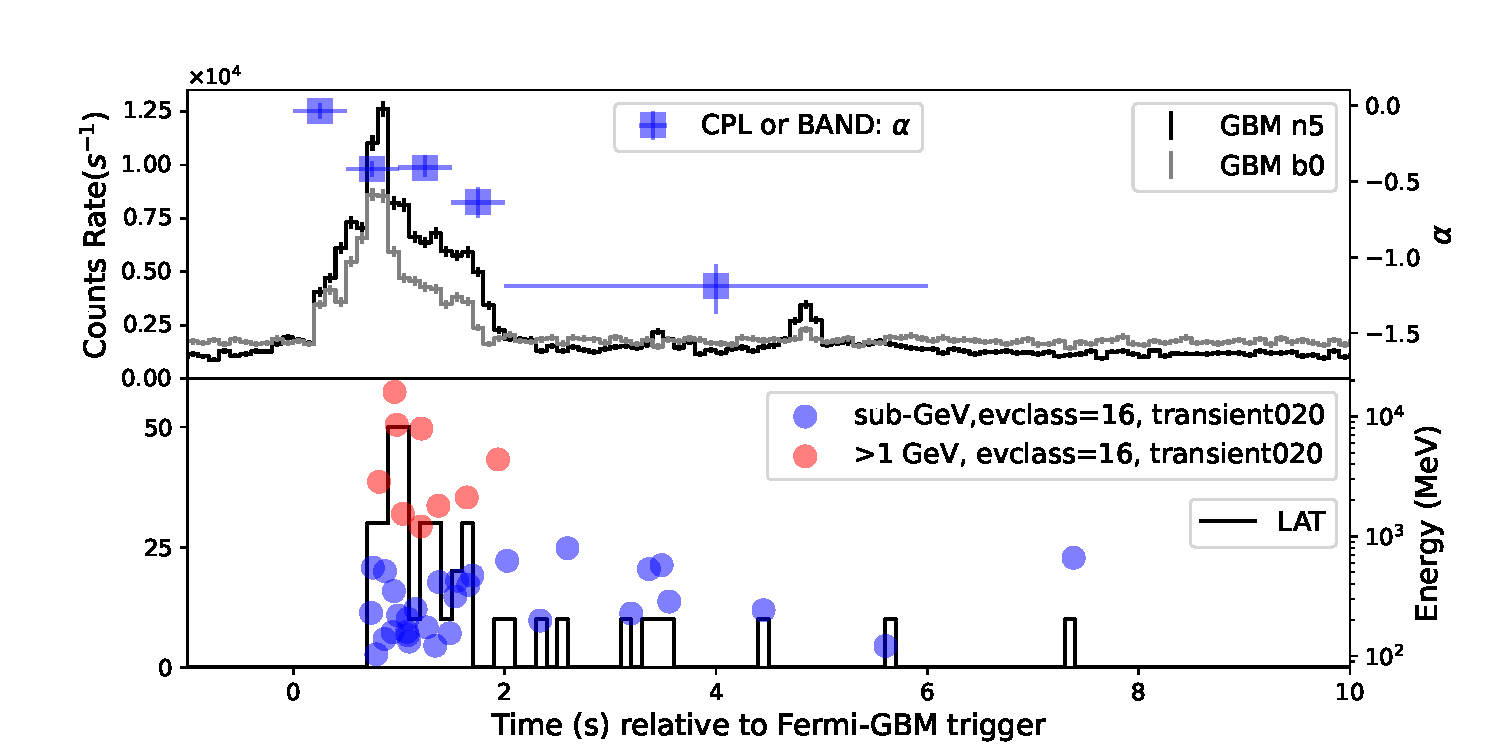
\includegraphics[width=.9\textwidth]{multi3.pdf}\put(-110,170){(a) }\\
%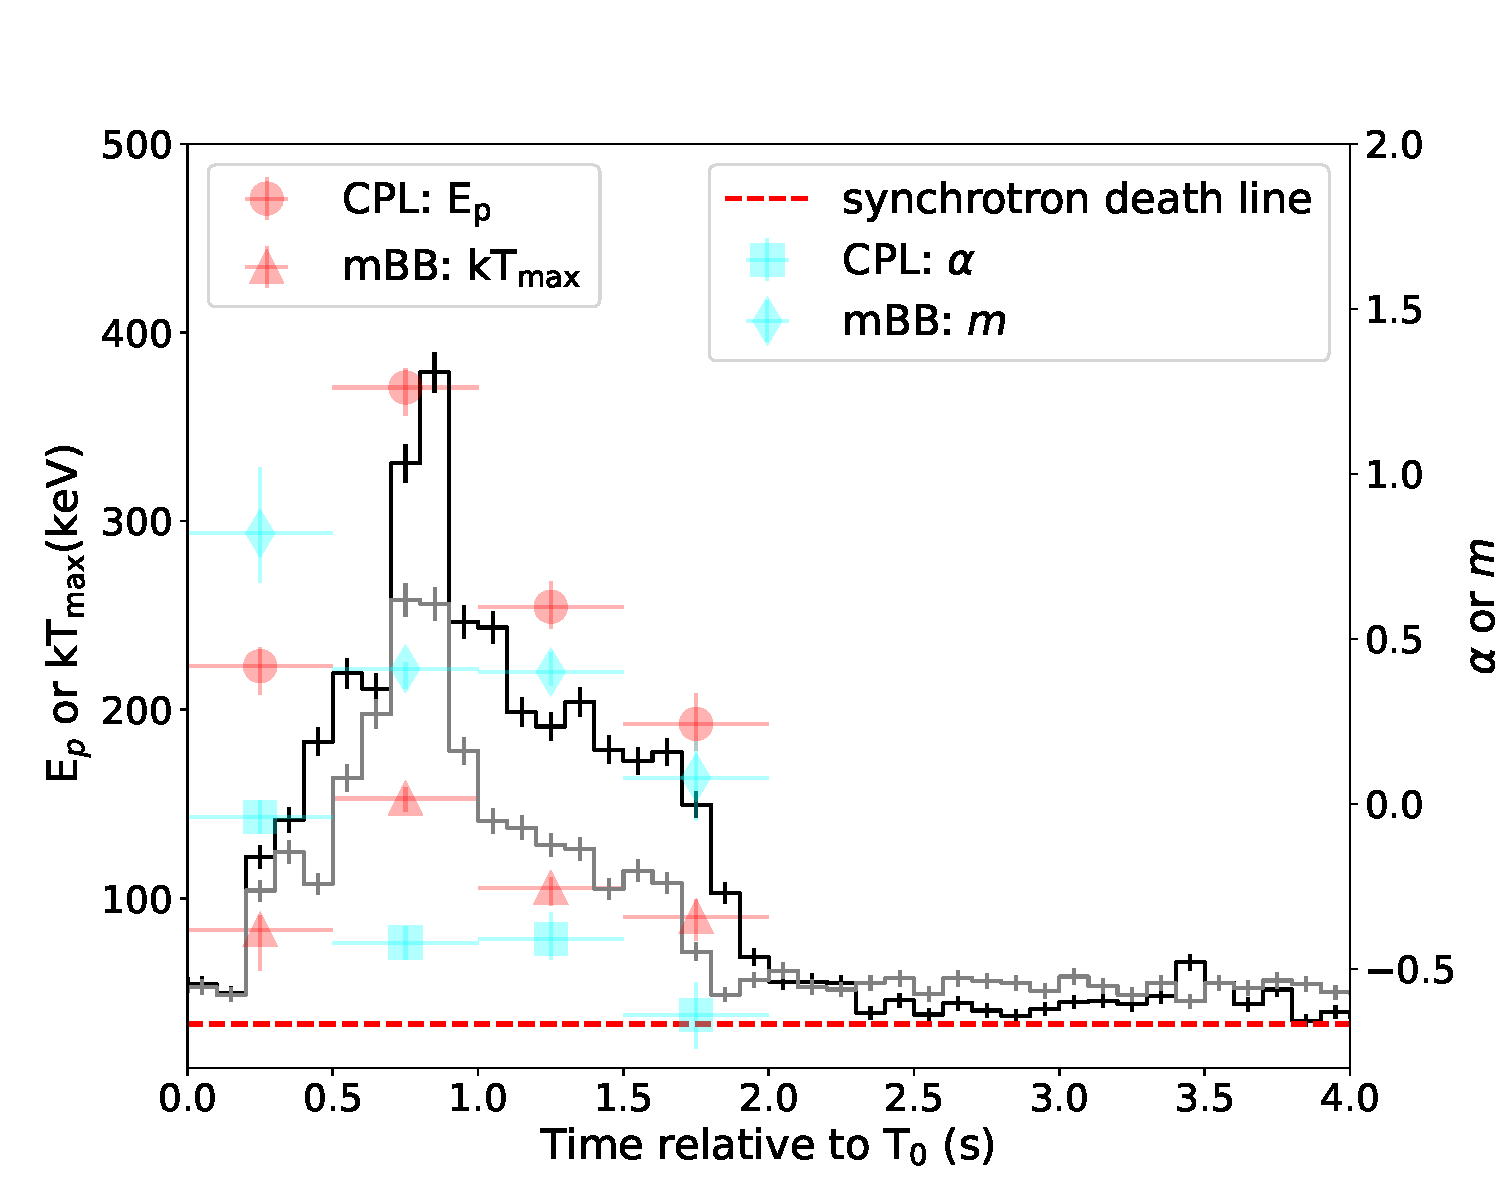
\includegraphics[width=.49\textwidth]{GRB210704_alphaEp.pdf}\put(-80,160){(b) }\\
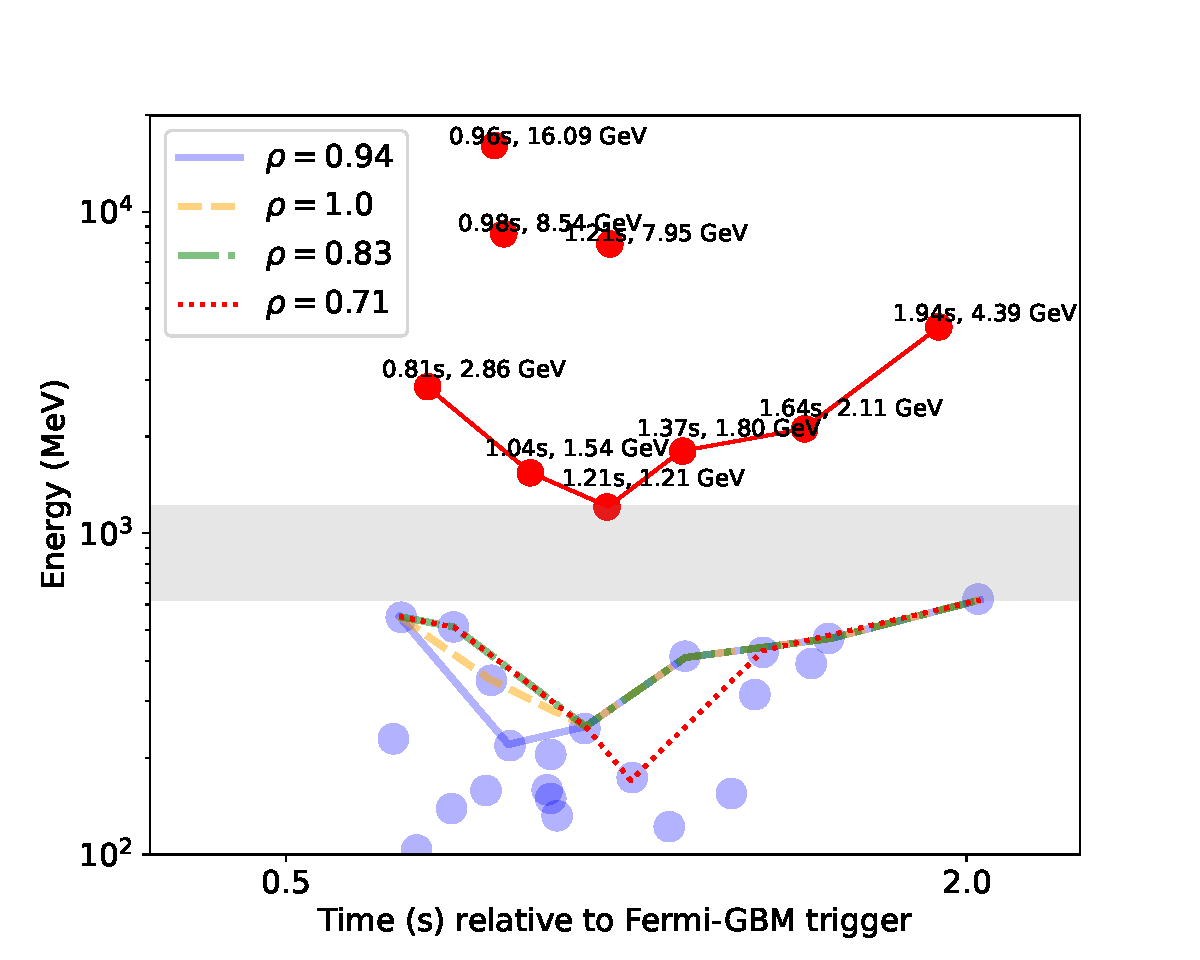
\includegraphics[width=.90\textwidth]{EvsT_LAT0p5_2p2_2.pdf}\put(-80,190){(b) }\\
%\includegraphics[width=0.5\textwidth]{Radec.pdf}\put(-190,210){(b) }
\caption{ (a) The light curves of GBM detectors (NaI 5 and BGO 0, upper plot) and LAT (bottom plot). The energy versus time of events with Fermi-LAT data of TRANSIENT020 (evclass=16). $\alpha$ values extracted in modeling results with  CPL (or BAND) function are denoted by blue squares with errors. 
%The modeling results with mBB (+PL), CPL and BAND function, including the evolution of $\alpha$, the peak energy of the $\nu F_{\nu}$ spectrum $E_{\rm p}$ and the parameters of mBB ($m$, $kT_{\rm max}$, $\alpha_2$).  
 (b) The Spearman rank correlation coefficient ($\rho$) of temporal evolution between $\gamma^{\rm envelop}_{\rm GeV}$ and $\gamma^{\rm envelop}_{\rm sub-GeV}$ (denoted by different line styles and colors) extracted with different bin-edge division ratio. The gray shadow between [0.62, 1.21] GeV shows the gap between sub-GeV and GeV photons.) \label{fig:observation}}
 \end{center}
\end{figure*} 



\section{Analysis on the anomaly in prompt high-energy emission}\label{sec:ana}
\subsection{The probability study of the gap }\label{sec: probstudy}
It is natural to conclude that high-energy emission could be described by a PL function since the production of GeV photons is much lower than that of sub-GeV photons, although they are reconstructed with a larger acceptance. However, it is necessary to investigate whether the gaps between them could be interpreted as statistical fluctuations. 
The energy spectrum is assumed to be described by a PL function with index $p$, 
\begin{equation}\label{func:PL}
N_{\rm PL}(E)=A E^{-p}.
\end{equation}
$p\simeq-1.7$ and time-averaged flux of $1.8\times10^{-5}$ erg cm$^{-2}$ s$^{-1}$ is determined in the modeling with high-energy data from $T_0+0.7$ s to 2.0 s.


To perform a hypothesis testing for the PL modeling of the high energy emission, \textit{the null hypothesis} is set to be that the statistical fluctuation could account for the gap of $[0.62,1.21]$ GeV; the test statistic is maximum gaps below an upper limit of $E_{\rm up}=1.21$ GeV. %, as listed below；
%\begin{itemize}
%    \item probabilities of the maximum gap $\mathrm{Prob_{\rm gap, max}}$;
%    \item maximum gaps below an upper limit of $E_{\rm up}=1.21$ GeV.
%\end{itemize}
A Monte-Carlo (MC) simulation is performed and $1.4\times10^5$ samples of the same total number of photons are generated based on the TI spectrum of real data in $T_0+[0.70,2.05]$ s; note that the folded model with the response from the detector is used. The probability density (PD) distribution of the maximum gaps is extracted, as shown in Figure~\ref{fig:maxEobsGeV_dTin} (a). The probability of a gap width of $\geq590$ MeV for photons below 1.21 GeV is determined to be $<10^{-3}$, thus \textit{the null hypothesis} that statistical fluctuation could explain the gap of $[0.62,1.21]$ GeV is rejected at a level of significance of $\alpha=0.001$, or the corresponding p-value is 0.001. 


In fact, considering the smoothing effect of the TI spectrum on the gap, the p-value for the gap is overestimated in the case of TI analysis, because the gap width varies with time, and that in the TI spectrum it is the intersection of all, which is the smallest. In TR analysis, the expected number of photons in the folded model in the energy bins (with index $i$) of gaps for each slice (with index $s$) is denoted as $N^{\mathrm{mod}}_{i,s}$. The probability of the gap due to the statistical fluctuation is derived as
\begin{equation}
\mathrm{Prob_{\rm gap}}=\prod_s \prod_i f(N^{\mathrm{mod}}_{i,s}, N^{\mathrm{obs}}_{i,s}),   
\end{equation}
where $f(N^{\mathrm{mod}}_{i,s}, N^{\mathrm{obs}}_{i,s})$ is the Poisson probability with expected mean values of $N^{\mathrm{mod}}_{i,s}$, which are determined by modeling. Note that in the modeling, the energy bins, including the zero-count bins in gaps, are all used, thus $\rm Prob_{\rm gap}$ is determined conservatively. 

Table~\ref{tab:gapprob} shows the results of TR analysis. The index of TI modeling with an PL is fixed to that of TI modeling. The lowest level of significance is $6\times10^{-4}$, which is less than that of the TI analysis; $\rm Prob_{\rm gap}$ between GeV and sub-GeV is determined to be less than $5\times10^{-6}$, which is very small. Note that the other gaps among the GeV photons have a much larger probability of $\sim10^{-2}$, which implies that emission above the gap is not inconsistent with \textit{the null hypothesis}.
\begin{figure*}
\begin{center}
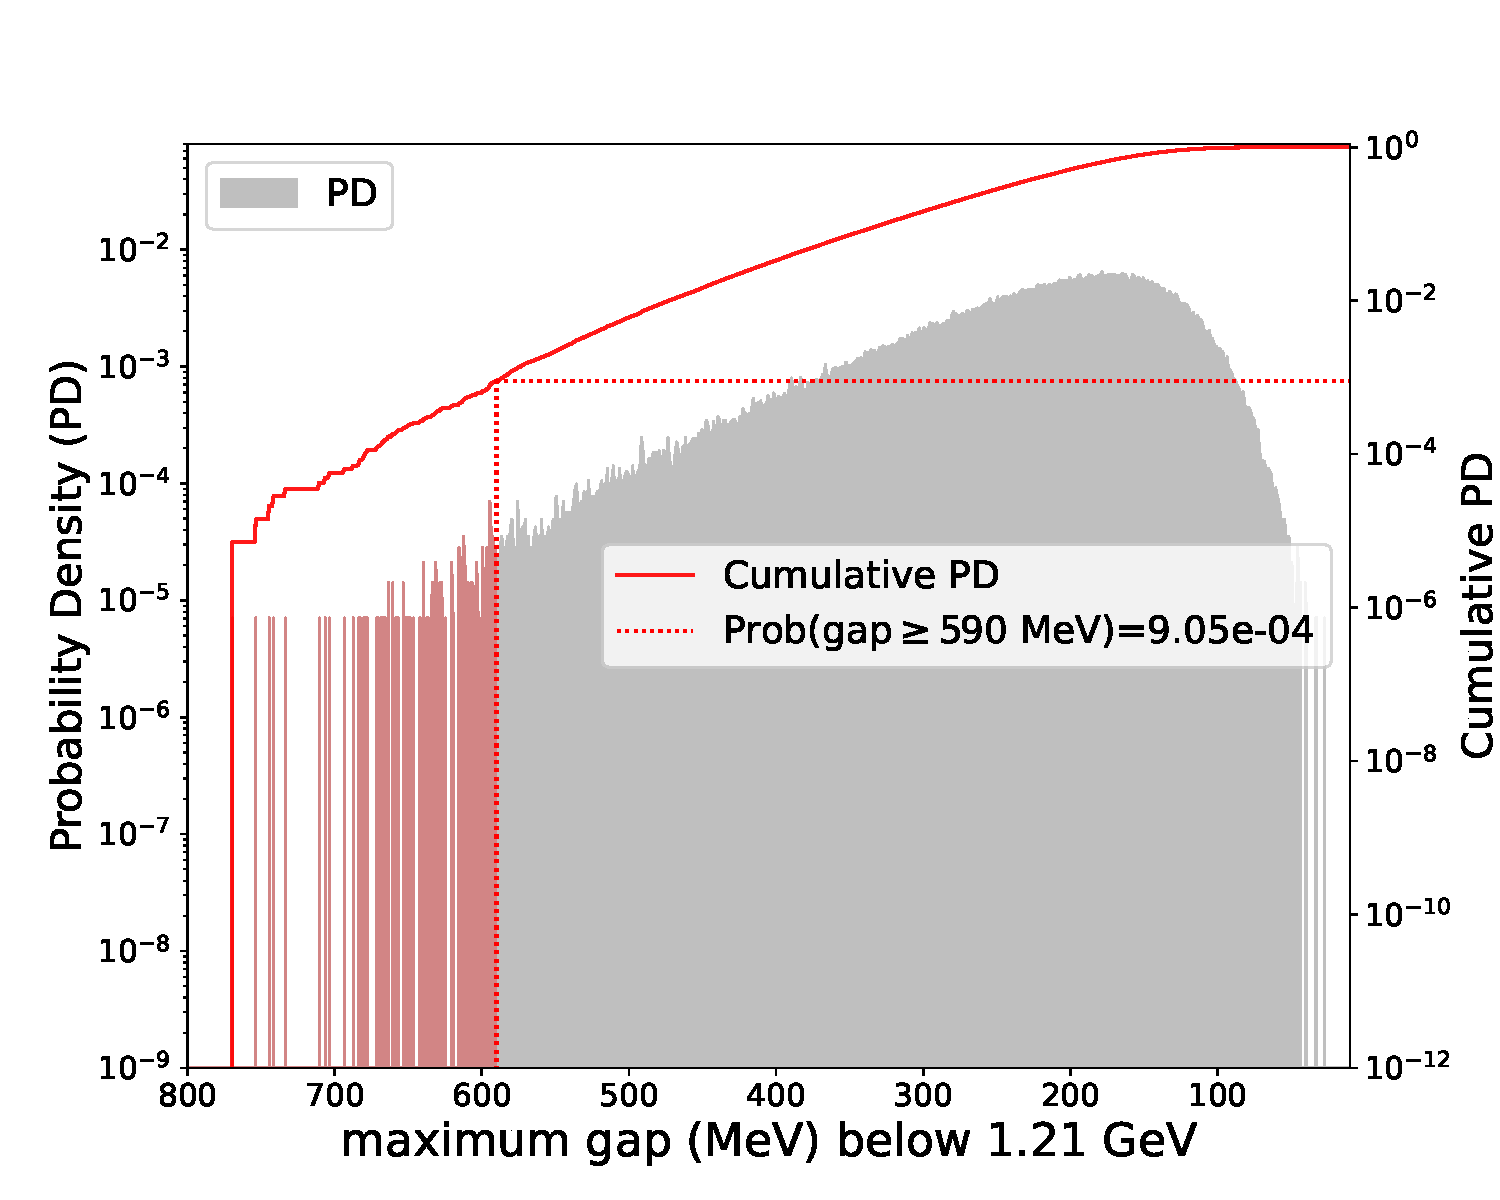
\includegraphics[width=.5\textwidth]{gapdis_hist_siglevel.pdf}\put(-80,160){(a) }
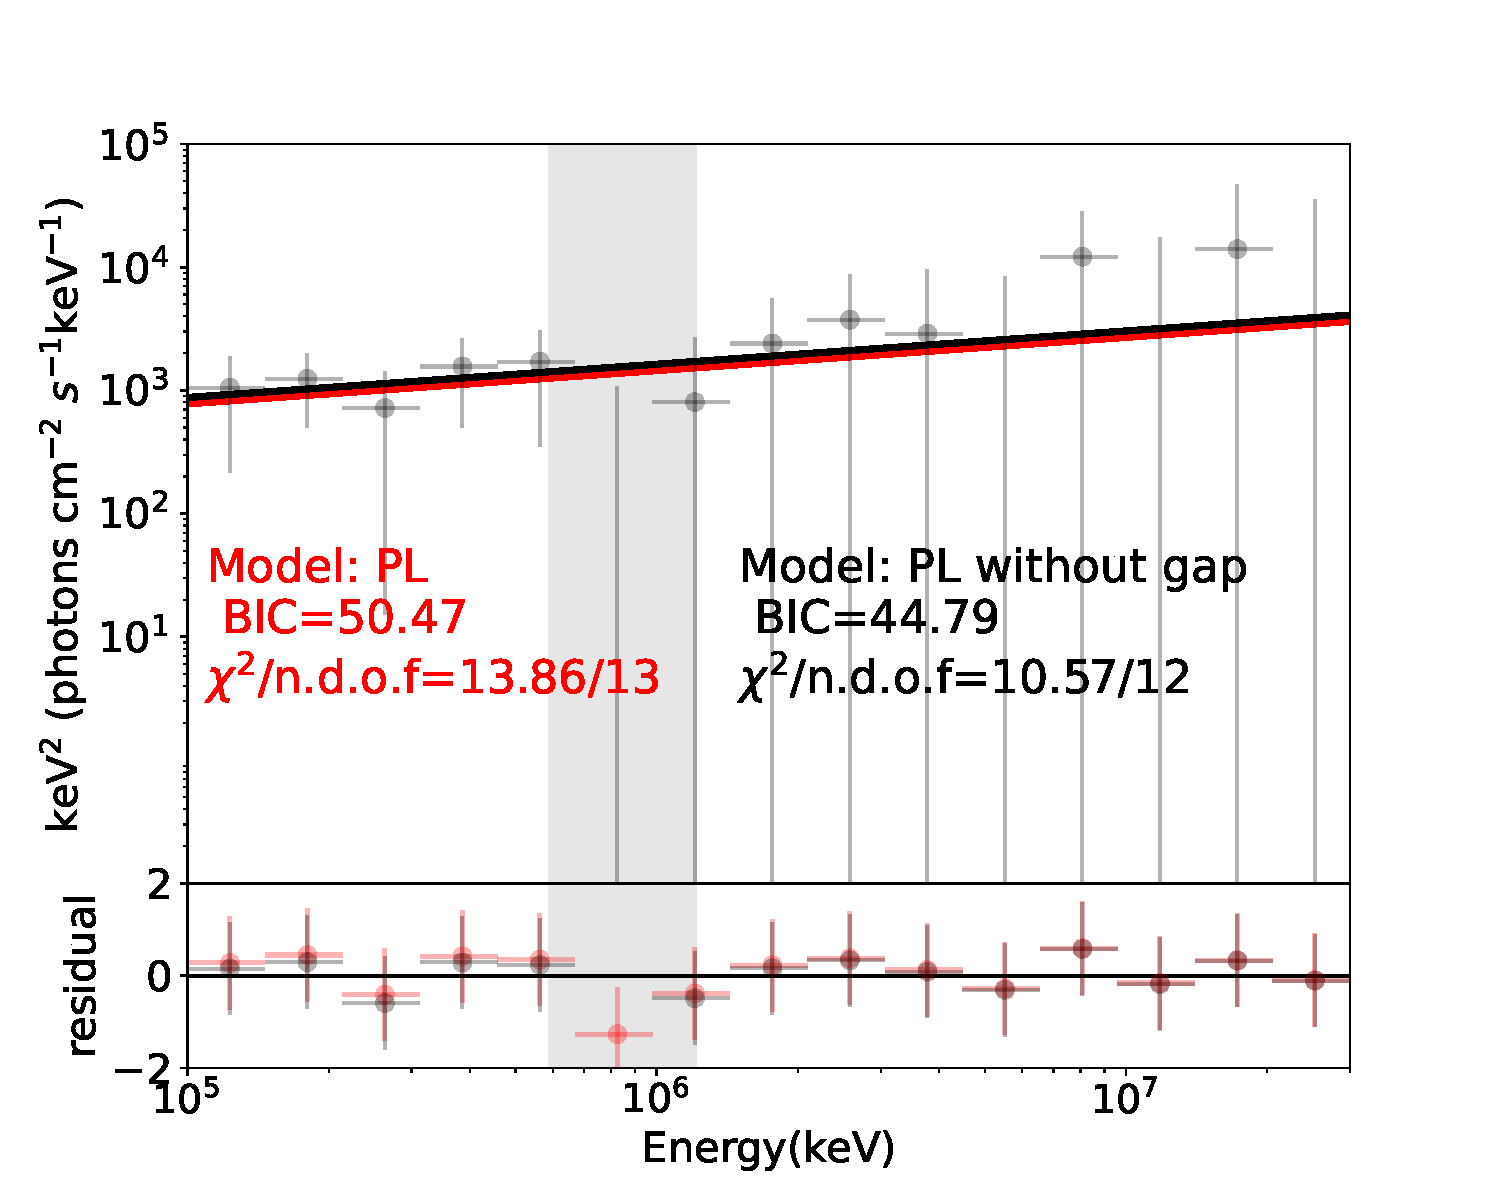
\includegraphics[width=.5\textwidth]{Fv_PL0_GRBHEB210704.pdf}\put(-50,160){(b) }\\
\caption{ (a) PD and cumulative PD of gaps in photons below 1.21 GeV. (b) The spectral modeling with and without the gap bin. 
\label{fig:maxEobsGeV_dTin}}
 \end{center}
\end{figure*} 

\begin{deluxetable*}{lccccc|c}
%\tabletypesize{\tiny}
\tabletypesize{\small}
\tablewidth{0pt}
\tablecaption{Time-resolved p-values and Poisson probabilities with assuming the gaps as the statistical fluctuations.\label{tab:gapprob}}
\tablehead{ 
\colhead{Time bins (s)}
&\colhead{[0.7, 0.9]}
&\colhead{[0.9, 1.2]}
&\colhead{[1.2, 1.4]}
&\colhead{[1.4, 1.65]}
&\colhead{[1.65, 2.05]}
&\colhead{$\prod_s \prod_i f(N^{\mathrm{mod}}_{i,s}, N^{\mathrm{obs}}_{i,s}=0)$}\\
\colhead{Gap range (MeV) between sub-GeV and GeV}&\colhead{[2860, 550]}&\colhead{[1540, 350]}&\colhead{[1210, 410]}&\colhead{[2110, 430]}&\colhead{[4390, 620]}
}
\startdata
 index $p$ fixed to TI results & & &$1.74\pm{0.10}$&&&\\
 p-value &0.0037 &0.0006 &0.018 &0.0067 &0.0034 \\
$N^{\mathrm{mod}}_{i,s}$, $f(N^{\mathrm{mod}}_{i,s},N^{\mathrm{obs}}_{i,s}= 0)$ of gap  &2.23,0.107&4.9,0.007&1.99,0.137&1.68,0.186&1.51,0.22&$4.5\times10^{-6}$\\
$N^{\mathrm{mod}}$ and $f$  above GeV-line &0.72,0.489&2.38,0.262&1.61,0.322&0.64,0.525&0.3,0.741&$1.6\times10^{-2}$\\\hline
\enddata
\end{deluxetable*}


\subsection{The possible correlation between  $\gamma^{\rm envelop}_{\rm sub-GeV}$ and $\gamma^{\rm envelop}_{\rm GeV}$}\label{sec: correlation}

The Spearman rank correlation coefficient ($\rho$)~\citep{spearman}\footnote{The spearman rank correlation coefficient $\rho$ is defined as $\rho = \frac{\mathrm{cov}(r(x),r(y))}{\sigma_x \sigma_y} $ where $r(a)$ represents the rank of element $a$. For non-duplicated datasets, $\rho$ can be interpreted as $\rho = 1 - \frac{6 \Sigma d^2_i}{n(n^2-1)} $ where $d_i = r(x) - r(y)$.} is used to quantify the monotonic relationship of the temporal evolution between the energy of $\gamma^{\rm envelop}_{\rm GeV}$ and that of $\gamma^{\rm envelop}_{\rm sub-GeV}$. %This nonparametric approach provides a robust correlation measure that is insensitive to outliers and does not rely on linear assumptions
In order to ensure a consistent one-to-one correspondence between data points, the energy envelope of sub-GeV photons was extracted as follows: each time point of GeV photons is defined in a bin, and the maximum sub-GeV energy value in that bin was adopted. To reduce the impact of artificial selection, different edges of the bin are traversed in this procedure. The bin edges are determined as follows: 1) the width of the first and the last edges' include most of the GeV and sub-GeV photons (far away points are excluded); 2) the inner edges are determined to be the n-equal diversion points in time of each adjacent lined GeV points; 3) the bin-edge division ratio (rate) is tested from 0.01 to 0.99 with an increment of 0.01 (for example, a rate equal to 0.2 means left five-division point). 

From all binning methods, four different energy envelopes of sub-GeV photons are extracted, as shown in Figure.~\ref{fig:observation} (c). $\rho$ is determined to be $> 0.7$ according to the minimal result of all sets of bin edges, which implies a strong correlation between $\gamma^{\rm envelop}_{\rm sub-GeV}$ and $\gamma^{\rm envelop}_{\rm GeV}$.\footnote{The grading standards and the corresponding correlation degrees are available online:~\href{https://www.statstutor.ac.uk/resources/uploaded/spearmans.pdf}{Spearman's correlation}. }

\subsection{TI spectral modeling with and without gap}\label{sec: modeling}
 The gap is statistically significant as analyzed in Section~\ref{sec: probstudy}. To further confirm this conclusion, modelings are performed with and without considering the gap in the model. However, the statistic is not large enough to extract the parameters of a specific physical model (e.g., an absorption line described by a gaussian function); moreover, the center energy and width of the gap vary with time, as shown in Fig~\ref{fig:observation} (c). Thus, the result of modeling with the gap subtracted in the bin is compared with that of all bins.
The Markov Chain Monte Carlo (MCMC) fitting is performed to find the parameters with maximum likelihood. The Sampling tool is $emcee$~\citep{2013PASP..125..306F}. \cite{2016MNRAS.463.1144W} suggested a Bayesian information criterion (BIC$=-2\rm{ln} \mathscr{L} +\rm{ln} (N)n$, $\mathscr{L}$ denotes the likelihood
function for all these parameters based on a Bayesian prior, $\rm N$ is the number of data points, and $\rm n$ is the number of free parameters) as a tool for model selection; a model that has a lower BIC value than the others is preferred. 
As shown in Figure~\ref{fig:maxEobsGeV_dTin} (b), the extracted indices of PL function are similar in the modelings with and without the gap; $\Delta$BIC=5.7, the preference for the gap in the PL model is positive.\footnote{If the change of BIC between these two models, $\Delta$BIC is from 2 to 6, the preference for the model with the lower BIC is positive; if $\Delta$BIC is from 6 to 10, the preference for that is strong; and if $\Delta$BIC is above 10, the preference is very strong.}




  

\section{The physical interpretation}\label{sec:physical_interpretation}
To account for the gap and correlation between $\gamma^{\rm envelop}_{\rm sub-GeV}$ and $\gamma^{\rm envelop}_{\rm GeV}$, some physical interpretations could be proposed naturally: sub-GeV photons and GeV photons are not produced from the same mechanism (see the details in Section~\ref{sec: multi}); or the photons produced between $\gamma^{\rm envelop}_{\rm sub-GeV}$ and $\gamma^{\rm envelop}_{\rm GeV}$, are absorbed by some resonant nuclide or photon-photon pair production (see the details in Section~\ref{sec:absorption}). %In order to distinguish between possible interpretations, an estimate of $\Gamma$ is given in Section~\ref{sec:esti}.


 %A model-dependent approach~\citep[e.g.,][]{2015ApJ...801..103G,2024ApJ...961..137S} is performed to obtain the estimate of the Lorentz Factor. For GRB 210704A,
 

\subsection{The multi-component emission mechanism}\label{sec: multi}
 If the GeV photons are due to another mechanism that differs from that of sub-GeV photons, the evolution of $\Gamma$ may account for the correlation between $\gamma^{\rm envelop}_{\rm sub-GeV}$ and $\gamma^{\rm envelop}_{\rm GeV}$, since the energies of $\gamma^{\rm envelop}_{\rm sub-GeV}$ and $\gamma^{\rm envelop}_{\rm GeV}$ are both boosted with the same Lorentz Factor. 

GeV photons may be produced in re-scattered process by sub-GeV photons in the IC mechanism. In the Thompson regime, one has
\begin{equation}
E_{\rm IC, obs}\simeq\Gamma\gamma'^{2}_e E'_{\rm seed}/(1+z),    
\end{equation}
 where the energy ratio of re-scattered photons to sub-GeV ones that are only scattered once is $\gamma_e^{'2}$; $\gamma_e^{'2}$ is estimated to be about 5 from the observation of (2.86 GeV, 0.55 GeV) and (1.21, 0.25) GeV. However, for the production of sub-GeV photons, $E'_{\rm seed }\sim 500$ keV is too energetic for seed photons in the comoving frame and Thompson regime. 
 In the Klein-Nishina (KN) regime, re-scattered photons cannot gain more energy via multi-time scattering. 
 Thus, multi-scattering can hardly explain the anomaly.

 



 
 


\subsection{The Resonant Nuclide Absorption Scenario and Other Potential Absorption Mechanism}
\label{sec:resonant-nuclide-absorption}\label{sec:absorption}

\textit{Energy scale.}---Applying the Doppler correction $E' \approx E_{\rm obs} (1+z) / 2\Gamma$, where $z \simeq 0.27$ is the redshift derived from the Amati relation and jet modeling \cite{2023MNRAS.522.5204B}, the observed gap of $0.6-1.2$ GeV translates to a comoving energy range of:
\begin{equation}
E_{\rm gap}^{\prime} \approx 2 - 7 \text{ MeV},
\end{equation}
where the lower (upper) limit corresponds to 0.55 (2.86) GeV and $\Gamma\simeq 280$(260). %Taking into account the robust and model-independent lower limit of $\Gamma\sim 160$ determined by $\gamma_{16.1 \rm GeV}$ and the maximum upper limit of the gap (2.86 GeV), $E_{\rm gap}^{\prime}$ cannot exceed 10 MeV. 

%A PL (or multi-energy-band PL) function with a nuclide absorption line could naturally explain the gaps and correlation between $\gamma^{\rm envelop}_{\rm sub-GeV}$ and $\gamma_{\rm 1-5GeV}$ without any additional mechanism or condition. 

%Taking into account the estimate of $\Gamma$ and the energy of gaps, The possible energy of the absorption line ranges from 4 MeV to 7 MeV in the comoving frame of the outflow. This aligns with laboratory-measured resonance levels of Fe-group nuclides (e.g. $^{56}\text{Fe}$, $^{52}\text{Cr}$)~\footnote{see the details on the web page of \href{https://www-nds.iaea.org/relnsd/vcharthtml/VChartHTML.html\#lastnuc=56Fe}{energy levels of nuclides}}. However, because of the large width of the gap, it is difficult to accurately identify the specific element. 

%---
%As shown in \cite{2020NDS...163..109K}, almost all the photonuclear absorption peaks are at $\sim$ 20 MeV; the only exception is for $^2$H, which is around 4 MeV, as given by the 1999 IAEA Photonuclear Data Library (IAEA/PD-1999)~\footnote{\href{https://www-nds.iaea.org/photonuclear/photonuclear99/}{https://www-nds.iaea.org/photonuclear/photonuclear99/}}
%Moreover, from the point of view of the r-process, $^2$H is the only possible nucleus that can be formed in a short period, which should be on the order of milliseconds. Other elements all need the $\beta$ decay to form, while the $\beta$ decay takes time on the order of minutes. 

%Resonant nuclide absorption is a physically plausible mechanism to explain key observational features of GRB 210704A, grounded in established nuclear physics and tight alignment with the data \citep{2006ApJ...642L.137R,2015ApJ...809..136K}. This scenario posits that high-energy photons are selectively absorbed by nuclei in the relativistic jet at discrete energies matching Doppler-shifted nuclear resonance levels, naturally producing the observed discrete spectral gaps—an effect distinct from the continuous spectra of leptonic/hadronic emission mechanisms. It further accounts for the synchronized temporal evolution of gap center energies, as the jet’s global Lorentz factor ($\Gamma$) governs the Doppler shift of all nuclear resonance energies (via $E_{\text{obs}} = (1+z)\Gamma E_{\text{rest}}$), leading to coordinated shifts across sub-GeV and GeV bands.



 %\citep{2006ApJ...642L.137R,2024ApJ...968L...5W}.

%Quantitative consistency is reinforced by inferred rest-frame resonance energies (~4–7 MeV) from observed gap energies (150 MeV–8 GeV) and plausible $\Gamma$ values (100–300), which align with laboratory-measured resonance levels of Fe-group nuclides (e.g., $^{56}\text{Fe}$, $^{52}\text{Cr}$) \citep{2006ApJ...642L.137R,2024ApJ...968L...5W}. The presence of such nuclides in GRB outflows is physically viable, as LGRB progenitors (massive stars) enrich their surroundings with heavy elements via stellar winds \citep{2019LRR....23....1M}, further supporting the scenario’s feasibility.

%\subsection{Other Potential Absorption Mechanisms}
%No alternative absorption mechanisms can simultaneously explain GRB 210704A’s discrete spectral gaps and synchronized gap evolution. Plasma absorption (via Langmuir oscillations) produces continuous spectral cutoffs or broad absorption bands, not sharp discrete gaps, with absorption energies tied to local plasma density—unable to drive coordinated gap evolution across sub-GeV/GeV bands \citep{2008FrPhC...3..306F}. Compton absorption (photon scattering by free electrons) causes smooth, energy-dependent attenuation rather than discrete features, as its efficiency scales continuously with photon energy \citep{2015ApJ...809..136K}. 

%Photon-photon pair production ($\gamma+\gamma \to 
%e^+ + e^-$) induces continuous high-energy cutoffs, not discrete gaps, and its energy threshold depends on local photon density—incapable of replicating the synchronized temporal trend of gap centers \citep{2010MNRAS.407.1033B}. Dust absorption, irrelevant to GRB outflows (hot, ionized environments preclude dust survival), only causes broadband extinction, not sharp energy-selective gaps \citep{2019LRR....23....1M}. All alternative mechanisms fail to satisfy both core observational constraints, suggesting resonant nuclide absorption as a viable explanation.

%Discussion & Summary

We propose that the gap arises from the resonant absorption of photons by nuclei entrained in the jet. The comoving energy of $\sim 4$ MeV aligns remarkably well with the photodissociation threshold of deuterium:
\begin{equation}
\gamma + {^2\text{H}} \rightarrow p + n.
\end{equation}
The binding energy of deuterium is 2.22 MeV. However, the cross-section for photodissociation peaks slightly above the threshold, typically around $4-5$ MeV \citep{IAEA2000}, which perfectly matches our derived comoving energy $E_{\rm gap}^{\prime}$.

Crucially, this energy scale distinguishes deuterium from all other potential nuclear absorbers. Heavier nuclides, particularly the Fe-group elements often invoked in supernova models, interact with photons primarily through the Giant Dipole Resonance (GDR). The GDR peak energy for nuclei with mass number $A$ is approximately $E_{\rm GDR} \approx 31.2 A^{-1/3} + 20.6 A^{-1/6}$ MeV \citep{1975RvMP...47..713B}, which places the resonance at $15-25$ MeV for heavy elements (e.g., $^{56}$Fe) \citep{2020NuDS..163..109K}. Such an absorption would manifest at observed energies $>3$ GeV, far above the gap detected in GRB 210704A. The unique low-energy threshold of deuterium makes it the only viable candidate for an absorption feature at $\sim 4$ MeV.

\textit{Timescales and Nucleosynthesis.}---The identification of deuterium is further supported by the dynamical timescales of the GRB jet. %ref
The dynamical time in the comoving frame is extremely short, on the order of hundreds of seconds:
\begin{equation}
t'_{\rm dyn} \approx \Gamma t_{\rm obs}/(1+z) \sim 300 \text{ s},
\end{equation}
where $t_{\rm obs} \sim 1 \text{s}$ is the time in the observer's frame.
In a neutron-rich outflow ejected from a merger, nucleosynthesis begins with the rapid capture of neutrons by protons ($p + n \rightarrow {^2\text{H}}$). To form heavier r-process elements (up to Lanthanides), the chain must proceed through seed nuclei creation. However, the formation of seeds heavier than deuterium is rate-limited by weak interactions ($\beta$-decays), which typically require timescales of seconds to minutes to proceed significantly.

Given the relativistic expansion, the jet material is ``frozen out" before significant quantities of heavy elements can form via $\beta$-decay. Consequently, the jet composition at the photospheric radius is expected to be dominated by nucleons and light isotopes, specifically deuterium, rather than heavy metals. This kinetic constraint robustly excludes Fe-group elements and reinforces the deuterium interpretation.



\textit{Other candidate absorption mechanism.}---As another candidate absorption mechanism, to generate an observed absorption with a center energy of $\sim1$ GeV, photon-photon pair production ($\gamma+\gamma \to 
e^+ + e^-$) requires a much larger Lorentz Factor, e.g. $\Gamma\gtrsim 1000$, than the estimate. Therefore, it is unlikely unless there exists sufficient evidence for an extremely large Lorentz Factor. 


\section{discussion and Conclusion }\label{sec:discussion}

\textit{Discussion.}---Let us demonstrate
the plausibility for the observation of photodissociation of deuterium in the jet of GRB 210704A as follows: the key point is if baryon loading in relativistic outflow could produce enough deuterium;
secondly, GeV photons are emitted with those in the resonant regions absorbed by deuterium, which requires that $\tau_{\gamma D}$ and $\tau_{\rm KN}$ should satisfy 
\begin{equation}\label{eq:criterion}
    \tau_{\rm KN}<1\lesssim\tau_{\gamma D}.
\end{equation}
at the emission radius ($R$) of high-energy photons, where the cross-section $\sigma_{\gamma D} \sim 2 \times 10^{-27}$ cm$^2$ and $n_D'$ is the comoving density of deuterium. 

%The detection of a deuterium absorption line implies significant baryon loading in the jet, specifically of neutron-rich matter; a high-entropy winds and fireballs associated with GRBs are proposed to be a source of light-element synthesis~\citep[e.g.][]{1967ARA&A...5..525F,2001ApJ...561..957P,2000ApJ...533..424O,2001ApJ...562..887T,2002ApJ...580..368P}.
The comoving density of the baryons is mainly contributed by protons, and can be expressed in terms of the isotropic energy of matter($E_{\rm m, iso}=L_{\rm m, iso} t_{\rm dur}$) is 
\begin{eqnarray}\label{eq:nbp}
     n^{\prime}_{b}&=&\frac{E_{\rm m, iso} }{4\pi R^2 (\frac{R}{\Gamma^2})  \Gamma m_p c^2}\nonumber\\
     &=&5.3\times 10^{21} (\frac{L_{\rm m, iso}}{10^{51}\ \rm erg \ \ s^{-1}})(\frac{R}{10^{11}\ \rm cm})^{-3} (\frac{\Gamma}{100})  \ \rm{cm^{-3}}, \nonumber\\
\end{eqnarray}
 where the shell width is $\sim R/\Gamma^2$ in time of $t_{\rm dur}$ in the lab frame~\citep{2018pgrb.book.....Z};\footnote{ In the following analysis, it is found that the emission of GeV photons in internal shock phase is reasonable.} $m_p c^2\simeq 1$ GeV is the mass of proton. The total luminosity of the outflow could be estimated by the radiative $L_{\gamma, \rm iso}$ and the radiative efficiency ($\epsilon_\gamma$), thus $L_{\rm m, iso}$ could be related to $L_{\gamma, \rm iso}$ as
\begin{equation}
    L_{\rm m, iso}\lesssim (1-\epsilon_\gamma)L_{\gamma, \rm iso}/\epsilon_\gamma. 
\end{equation}
For GRB 210704A, it is reasonable that $\epsilon_\gamma$ ranges from a few percents to nearly a half. This is because MeV prompt emissions are mainly photospheric, while the high-energy photons may be produced in the synchrotron by a group of relativistic electrons accelerated in internal shocks~\citep[e.g.,][]{2011ApJ...726...90Z,2008FrPhC...3..306F}. Thus we assume that $L_{\rm m, iso}$ is at least comparable with $L_{\gamma, \rm iso}\sim 10^{51}$ erg s$^{-1}$, or even tens of times larger.

The final mass fraction of deuterium ($Y_{D}$) can be greater than a few percent or even as large as $10\%$ in the case of $np$-decoupling occurring before it reaches at the radius of GeV emissions~\citep[see the simulation in ][]{2002ApJ...580..368P}. $n'_{D}$ is estimated to be:
\begin{equation}\label{eq:nDp}
   n^{\prime}_{ D}\sim n^{\prime}_{p} Y_{D}.
\end{equation}
 With Equations (\ref{eq:nbp})-(\ref{eq:nDp}), one has $\tau_{\gamma D}\gtrsim1$ at $R\sim10^{12-13}$ cm ($n^{\prime}_{D}(R)\sim10^{16}$ cm$^{-3}$ correspondingly). It is well consistent with the observation that the GeV photons have a very small time delay ($\Delta t$) relative to the MeV photons (mainly emitted at radius $R_{\rm ph}$)\footnote{$R_{\rm ph}\simeq10^{11}$ cm is estimated to be 
 \begin{eqnarray}
    R_{\rm ph}&\simeq&(\frac{L_{\rm m,iso}\sigma_{\rm T}}{8\pi m_pc^3\Gamma})^{1/3} r_0^{2/3}\nonumber\\
    &=&3.9\times10^{10} (\frac{L_{\rm m,iso}}{10^{51} \ \rm erg \ s^{-1}})^{1/3} (\frac{\Gamma}{100})^{-1/3}(\frac{r_0}{10^8\ \rm cm})^{2/3} \ \rm cm \nonumber
 \end{eqnarray}
 with the shell width $\simeq c\Delta t$ in the accelerating phase; if the outflow is already in the coasting phase before it reaches $R_{\rm ph}$,  $R_{\rm ph}\simeq 5.9\times10^{12}\frac{L_{\rm m,iso}}{10^{52}\ \rm erg \ s^{-1}} (\frac{\Gamma}{100})^{-3}$ cm, is of the same order~\citep{2000ApJ...530..292M}.}   by 
 \begin{equation}
   R\sim R_{\rm ph} + 2c\Gamma^2\Delta t(1+z).  
 \end{equation}
 The baryon loading in the jet is calculated to be $f_{b}M_{\rm iso}\sim10^{-7}$ to $10^{-6}M_{\odot}$ by $E_{\rm m, iso}=\Gamma M_{\rm iso}c^2$ ~\citep[the typical beaming factor for short GRBs is $f_b\sim6\times10^{-3}$, see][]{2014ARA&A..52...43B}, which is a reasonable value for merger events~\citep{2019LRR....23....1M,2025PhRvD.111f3040S}.
 
 GeV photons are emitted with those in the resonant regions absorbed by deuterium, which requires that $\tau_{\gamma D}$ and the depth of Compton scattering for GeV photons in KN regime ($\tau_{\rm KN}\sim\frac{\sigma_{\rm KN} n'_{e}R}{\Gamma}$) should satisfy 
\begin{equation}\label{eq:criterion}
    \tau_{\rm KN}\lesssim \tau_{\gamma D}.
\end{equation}

%\begin{eqnarray}
%\tau_{ \gamma_{\rm MeV},e}\sim\frac{\sigma_{\rm T} n'_{e^\pm}R}{\Gamma}, \label{eq:tauph}\\
%\tau_{\rm KN}\sim\frac{\sigma_{\rm KN} n'_{e}R}{\Gamma},\\
%\tau_{\gamma D}\sim\frac{\sigma_{\gamma D} n'_ D R}{\Gamma}.
%\end{eqnarray}
Internal shocks are natural sites for the dissipation of the kinetic energy of a baryonic fireball~\citep[e.g.][]{1990ApJ...365L..55S,1992MNRAS.258P..41R,1993ApJ...405..278M,1994ApJ...430L..93R}. Note that in the outflow, assuming local electrical neutrality in the jet, $n'_{e}\simeq n'_p+n'_D$ and $\sigma_{\rm KN}=\frac{3}{8}\sigma_{\rm T}x^{-1}(\textmd {ln} 2x+ \frac{1}{2})$\citep{1986rpa..book.....R};\footnote{The other positive particles, e.g. $\alpha$ particles, are ignored; and the production of pairs $e^{\pm}$ is limited at the radius of GeV emission.} for relativistic electrons, $x$ is determined by
\begin{equation}
x \equiv \frac{\gamma_e' E'_{\gamma}}{m_e c^2},
\end{equation}
where $E'_{\gamma}\simeq 4$ MeV for the resonant energy-band, $\gamma_e'$ is the Lorentz factor of electrons in the comoving frame. The minimum of $\gamma_e'$, $\gamma_{\rm e, min}'$
could reach $10^{3.5}-10^6$ and has a PL distribution with an index of approximately -2.5~\citep[e.g.,][]{1995ApJ...455L.143S,1996ApJ...473..204S,2013ApJ...769...69B}.\footnote{$\gamma_{e,\rm min}'$  could be estimated as
\begin{equation}
\gamma_{\rm e,min}' \simeq 
\varepsilon_e\,\frac{p-2}{p-1}\,
\frac{m_p}{m_e}\,
(\gamma_{\rm ud}-1),
\end{equation}
where $\varepsilon_e$ is the fraction of energy transferred to electrons accelerated in shocks; $\gamma_{\rm ud}$ is the relative Lorentz factor between upstream and downstream regions, and it could be $\gg1$.
} Criterion (\ref{eq:criterion}) requires $\gamma_{e,\rm min}'\sim10^3$, which lies within theoretically acceptable range.




%For an observed energy of about 1 GeV, $x\sim5$, $\sigma_{\rm KN}\simeq0.2 \sigma_{\rm T}$, thus $\tau_{\gamma D}\sim10^{-3}\tau_{ \rm KN} $. This means that at the photosphere radius of the GeV photon emission, $\tau_{\rm KN}\sim1$ and $\tau_{\gamma D}$ has been less than 1. However, in reality, local electrical neutrality may not hold because of the existence of the magnetic field in the outflow, especially in the case of a rotation~\citep[e.g.,][]{2010ApJ...709.1100P,2021ApJ...906..105C}. In GRB 210704A, after $T_0+1.5$s to the extension to $T_0+6$ s, the non-thermal emission becomes dominant, which implies a considerable Poynting flux in the outflow. Assume a magnetic field energy ($E_{\rm B}\propto B^2$) could account for $\lesssim10\%$ of the total energy, $B$ is estimated to be $\sim10^{-12}$ T at the radius of prompt emission. In the plasma of the outflow, the radial drift velocity $\mathbf{v}'_{\rm d,r}\simeq\frac{u'_{\perp}}{eB^3}\mathbf{B_{\phi}}\times \nabla_{\rm z} B$ could cause a separation between electrons and positively charged particles, until an electromagnetic balance is supported. The internal energy $u’_{\perp}\simeq 1$ keV in the comoving frame corresponds to  $\mathbf{v}'_{\rm d,r}$ of the order of $10^{5}$ m s$^{-1}$ in the radius of prompt emission\footnote{For an arbitrary magnetic configuration before dissipation, $B_{\rm z}r_{\rm jet}^2\simeq$ const and  $B_{\phi}^2r_{\rm jet}^2\simeq$ const because of flux conservation~\citep{2018pgrb.book.....Z}.$u'_{\perp}\propto 1/R$, $B\sim 1/R$; $\mathbf{B_{\phi}}\times \nabla_{\rm z} B/B^2\propto 1/R$ in the acceleration phase of a fireball, thus v$_{\rm d, r}\propto 1/R$. Thus v$_{\rm d, r}$ should be larger than $10^5$ m s$^{-1}$ before prompt emission.}; if without considering the electromagnetic balance, it is large enough for a considerable separation ($\sim 0.01$ rad) in the opening angle during $t'_{\rm dyn}$ of a few hundreds of seconds, as calculated in ~\cite{2021ApJ...906..105C}. 
%In the region of positive charged particles, $\tau_{\gamma D}$ could be 
%A numerical simulation and calculation are beyond the scope of this article, and a rough calculation for the 


\textit{Conclusion.}---
We identified a statistically significant spectral gap in the prompt emission of GRB 210704A. Interpreting this as resonant absorption by deuterium nuclei in a jet with $\Gamma \sim 200-300$ for the first time, we find a consistent physical picture that links the burst to a neutron-rich progenitor. This represents the first direct spectroscopic detection of r-process nucleosynthesis ingredients in the prompt gamma-ray phase, opening a new window for studying nuclear astrophysics in extreme environments.


Previous studies of GRB 210704A noted its peculiar properties and suggested a compact object merger origin, despite its duration lying in the intermediate range \citep{2021GCN.30380....1M, 2023MNRAS.522.5204B}. Our finding provides a completely independent confirmation of this progenitor channel. Unlike kilonovae, which probe the sub-relativistic ejecta days after the event, this spectral feature probes the relativistic jet itself seconds after launch, revealing the initial chemical composition of the r-process flow.

%In this \textit{letter}, 





%This work presents three statistically robust phenomenological features of the prompt high-energy emission (100 MeV–10 GeV) from GRB 210704A, focusing exclusively on data-driven observations to provide a model-independent benchmark for future GRB research. Below, we contextualize these findings within existing GRB literature, validate their reliability, and outline limitations and future research directions, followed by a concise summary of core results.

% the key points (1, 2, 3) in introduction should be here

% from Mabq We present three statistically robust, unprecedented phenomenological features of GRB 210704A’s prompt high-energy emission (100 MeV–10 GeV): (1) discrete spectral gaps that cannot be attributed to statistical fluctuations; (2) a tight linear temporal correlation between the energy envelopes of sub-GeV and GeV emission, distinct from canonical high-energy delays; and (3) coordinated energy-dependent evolution of sub-GeV and GeV bands across the entire prompt phase. These features distinguish GRB 210704A from canonical GRBs and fill critical gaps in high-energy GRB observational data.

% from Mabq The core contribution of this work is a rigorous, model-independent observational benchmark that constrains the diversity of GRB prompt emission behaviors. By documenting these unique features, we provide a foundation for future studies—both observational (e.g., identifying similar GRBs) and theoretical (e.g., developing models consistent with the observed patterns)—to advance our understanding of extreme astrophysical transients.
 
%TC:ignore
%\iffalse
\begin{acknowledgements}
 The author thanks the support of the National Natural Science Foundation of China (grant No. 12303052) and XXXXX. The author is very grateful for the public GRB data from Fermi/GBM and Fermi/LAT.  Q. Liu and Dr X.Y. Song are very grateful for the support from China's Space Origins Exploration Program. Prof. Y.C. Zou, Prof. W.T. Deng and Prof. B.Q. Ma thank XXX. 
 %The author is very grateful to the suggestions and comments from Prof. Shuang-Nan Zhang. I thank Prof. Shuang-shi Fang for polishing the language in some paragraphs.
 %X.Y. Song is very grateful for the comments and suggestions from the anonymous referees and suggestions from Prof. Kin-Wang Ng on the combustion from NS to QS.
\end{acknowledgements}
%\fi
%\clearpage

%\clearpage
%TC:endignore
\bibliography{LIV}
\bibliographystyle{aasjournal}

\end{document}

% End of file `sample631.tex'.
